\section{Notions of linear separability}
\label{section:notions-of-linear-separability}

We define two notions of linear separability for multiclass classification. The
first notion is the standard notion of linear separability used in the proof of
the mistake bound for the \textsc{Multiclass Perceptron} algorithm\citep[see e.g.][]{Crammer-Singer-2003}. The second
notion is stronger, i.e. more restrictive. %However, it is more suitable for the
%bandit setting, since it allows for a simple and efficient algorithm; see
%Section~\ref{section:algorithm-for-strongly-linearly-separable-data}.

\begin{definition}
[Linear separability]
\label{definition:linear-separability}
Let $(V,\ip{\cdot}{\cdot})$ be an inner product space, $K$ be a positive
integer, and $\gamma$ be a positive real number.
We say that labeled examples $(x_1, y_1),
(x_2, y_2), \dots, (x_T, y_T) \in V \times \{1,2,\dots,K\}$ are
%said to be
\begin{enumerate}
\item
\emph{weakly linearly separable with a margin $\gamma$} if there exist vectors
$w_1, w_2, \dots, w_K \in V$ such that
\begin{align}
\label{equation:weak-linear-separability-1}
& \sum_{i=1}^K \norm{w_i}^2 \le 1 \; , \\
\label{equation:weak-linear-separability-2}
& \begin{gathered}
\forall t \in \{1,2,\dots,T\} \quad \forall i \in \{1,2,\dots, K\} \setminus \{y_t\} \\
\ip{x_t}{w_{y_t}} \ge \ip{x_t}{w_i} + \gamma \; ,
\end{gathered}
\end{align}
\item
\emph{strongly linearly separable with a margin $\gamma$} if there exist vectors
$w_1, w_2, \dots, w_K \in V$ such that
\begin{align}
\label{equation:strong-linear-separability-1}
& \sum_{i=1}^K \norm{w_i}^2 \le 1 \; , \\
\label{equation:strong-linear-separability-2}
& \forall t \in \{1,2,\dots,T\} \qquad \qquad \ip{x_t}{w_{y_t}} \ge \gamma/2 \; , \\
\label{equation:strong-linear-separability-3}
& \begin{gathered}
\forall t \in \{1,2,\dots,T\} \quad \forall i \in \{1,2,\dots, K\} \setminus \{y_t\} \\
\ip{x_t}{w_i} \le - \gamma/2 \; .
\end{gathered}
\end{align}
\end{enumerate}
\end{definition}

%The notion of weak linear separability is a standard assumption used in the
%full-information setting to upper bound the number of mistakes of the
%\textsc{Multiclass Perceptron} algorithm.
%%%%%
%(Recall our discussion on the topic in Section~\ref{section:introduction}.)
%Namely, \citet{Crammer-Singer-2003}
%prove that if the examples are weakly linearly separable with a margin $\gamma$
%and the norm of the examples is bounded by $R$, then \textsc{Multiclass
%Perceptron} algorithm makes at most $\left\lfloor 2(R/\gamma)^2 \right \rfloor$
%mistakes. It is a folklore result that \textsc{Multiclass Perceptron} is
%essentially optimal in the sense that any (possibly randomized) algorithm must
%make $\frac{1}{2} \left\lfloor (R/\gamma)^2 \right \rfloor$ mistakes in the
%worst case. For completeness, we state the \textsc{Multiclass Perceptron}
%algorithm, the upper and lower bound on the number of mistakes, and their proofs
%in Appendix~\ref{section:multiclass-perceptron-proofs} in the supplementary
%material.
%%%%%

The notion of strong linear separability has appeared in the literature; see
e.g.~\citet{Chen-Chen-Zhang-Chen-Zhang-2009}. Intuitively, strong linear
separability means that, for each class $i$, the set of examples belonging to
class $i$ and the set of examples belonging to the remaining $K-1$ classes are
separated by a linear classifier $w_i$ with margin $\frac{\gamma}{2}$.

It is easy to see that if a set of labeled examples is strongly linearly
separable with margin $\gamma$, then it is also weakly linearly separable with
the same margin (or larger). Indeed, if $w_1, w_2, \dots, w_K \in V$ satisfy
\eqref{equation:strong-linear-separability-1},
\eqref{equation:strong-linear-separability-2},
\eqref{equation:strong-linear-separability-3} then they satisfy
\eqref{equation:weak-linear-separability-1} and
\eqref{equation:weak-linear-separability-2}.

In the special case of $K=2$, if a set of labeled examples is weakly
linearly separable with a margin $\gamma$, then it is also strongly linearly
separable with the same margin. Indeed, if $w_1, w_2$ satisfy
\eqref{equation:weak-linear-separability-1} and
\eqref{equation:weak-linear-separability-2} then $w_1' = \frac{w_1 - w_2}{2}$,
$w_2' = \frac{w_2 - w_1}{2}$ satisfy
\eqref{equation:strong-linear-separability-1},
\eqref{equation:strong-linear-separability-2},
\eqref{equation:strong-linear-separability-3}.
Equation~\eqref{equation:strong-linear-separability-1} follows from
$\norm{w_i'}^2 \le (\frac{1}{2} \norm{w_1} + \frac{1}{2} \norm{w_2})^2 \le
\frac{1}{2}\norm{w_1}^2 + \frac{1}{2}\norm{w_2}^2 \le \frac{1}{2}$ for $i=1,2$.
Equations~\eqref{equation:strong-linear-separability-2}
and~\eqref{equation:strong-linear-separability-3} follow from the fact that
$w_1' - w_2' = w_1 - w_2$.

However, for any $K \ge 3$ and any inner product space of dimension at least
$2$, there exists a set of labeled examples that is weakly linearly separable
with a positive margin $\gamma$ but is not strongly linearly separable with
any positive margin.~\autoref{figure:weakly-linearly-separable-examples-with-margin}
shows one such set of labeled examples.

\begin{figure}
\begin{center}
 \scalebox{.8}{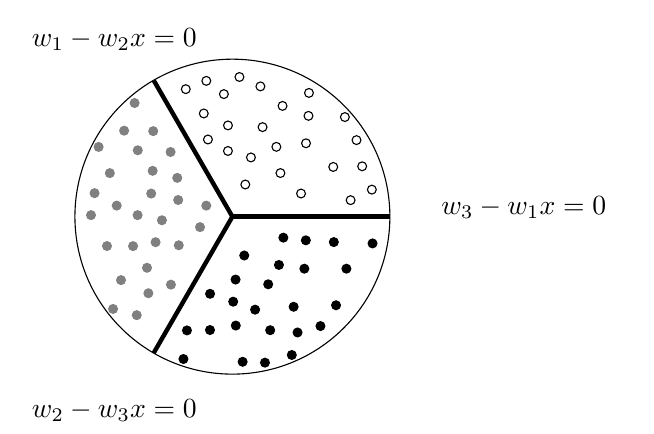
\begin{tikzpicture}[scale=0.4]

  \useasboundingbox (-6.5,-6) rectangle (12.5,6);
  % \draw[help lines] (-5.5,-5.5) rectangle (5.5,5.5);

  % Grid and coordinate axes
  %% \draw[help lines] (-5.2,-5.2) grid (5.2,5.2);
  %% \draw[thick, ->, >=latex] (-5.2,0) -- (5.2,0);
  %% \draw[thick, ->,  >=latex] (0,-5.2) -- (0,5.2);

  % Notable points
  \coordinate (Origin) at (0,0);

  \coordinate [label={[xshift=-5mm, yshift=2.5mm]$\ip{w_1 - w_2}{x} = 0$}] (A) at (120:5);
  \coordinate [label={[xshift=-5mm, yshift=-10mm]$\ip{w_2 - w_3}{x} = 0$}] (B) at (240:5);
  \coordinate [label={[xshift=+17mm, yshift=-1.5mm]$\ip{w_3 - w_1}{x} = 0$}] (C) at (360:5);

  % Circle which contains all the examples.
  \draw (Origin) circle (5);

  \draw[ultra thick] (Origin) -- (A);
  \draw[ultra thick] (Origin) -- (B);
  \draw[ultra thick] (Origin) -- (C);

  % Class 0 points. Angles between 0.0 and 120.0
  \draw[color=black, fill=none]
                    (7.94:3.79) circle (4pt)
                    (10.97:4.51) circle (4pt)
                    (18.63:2.30) circle (4pt)
                    (21.20:4.42) circle (4pt)
                    (26.23:3.57) circle (4pt)
                    (31.66:4.63) circle (4pt)
                    (41.52:4.77) circle (4pt)
                    (42.22:2.06) circle (4pt)
                    (44.90:3.30) circle (4pt)
                    (52.95:4.01) circle (4pt)
                    (57.79:2.62) circle (4pt)
                    (58.25:4.62) circle (4pt)
                    (65.64:3.86) circle (4pt)
                    (68.11:1.10) circle (4pt)
                    (71.38:3.00) circle (4pt)
                    (72.60:1.97) circle (4pt)
                    (77.86:4.23) circle (4pt)
                    (87.11:4.44) circle (4pt)
                    (92.77:2.90) circle (4pt)
                    (93.88:2.09) circle (4pt)
                    (93.97:3.90) circle (4pt)
                    (100.87:4.39) circle (4pt)
                    (105.50:3.40) circle (4pt)
                    (107.58:2.57) circle (4pt)
                    (110.09:4.31) circle (4pt)
                    ;

  % Class 1 points. Angles between 120.0 and 240.0
  \draw[color=gray, fill=gray]
                    (130.71:4.76) circle (4pt)
                    (132.80:3.70) circle (4pt)
                    (133.71:2.84) circle (4pt)
                    (141.55:4.39) circle (4pt)
                    (144.89:2.14) circle (4pt)
                    (144.96:3.67) circle (4pt)
                    (150.11:2.92) circle (4pt)
                    (152.47:4.79) circle (4pt)
                    (157.09:0.90) circle (4pt)
                    (160.45:4.13) circle (4pt)
                    (162.92:1.80) circle (4pt)
                    (164.13:2.68) circle (4pt)
                    (170.32:4.44) circle (4pt)
                    (174.55:3.69) circle (4pt)
                    (179.08:3.01) circle (4pt)
                    (179.39:4.49) circle (4pt)
                    (182.94:2.24) circle (4pt)
                    (193.19:4.09) circle (4pt)
                    (196.53:3.29) circle (4pt)
                    (197.93:1.08) circle (4pt)
                    (198.39:2.57) circle (4pt)
                    (208.08:1.93) circle (4pt)
                    (209.68:4.07) circle (4pt)
                    (210.92:3.16) circle (4pt)
                    (217.72:4.79) circle (4pt)
                    (222.35:3.61) circle (4pt)
                    (225.84:4.36) circle (4pt)
                    (227.89:2.91) circle (4pt)
                    ;

% Class 2 points. Angles between 240.0 and 360.0
  \draw[color=black, fill=black]
                    (248.23:3.89) circle (4pt)
                    (251.03:4.78) circle (4pt)
                    (253.86:2.55) circle (4pt)
                    (258.82:3.67) circle (4pt)
                    (270.54:2.70) circle (4pt)
                    (271.79:3.46) circle (4pt)
                    (272.88:2.00) circle (4pt)
                    (274.04:4.62) circle (4pt)
                    (282.58:4.75) circle (4pt)
                    (283.72:3.04) circle (4pt)
                    (286.97:1.29) circle (4pt)
                    (288.41:3.80) circle (4pt)
                    (293.24:4.78) circle (4pt)
                    (297.90:2.43) circle (4pt)
                    (299.36:4.22) circle (4pt)
                    (304.20:3.46) circle (4pt)
                    (308.83:4.46) circle (4pt)
                    (313.94:2.13) circle (4pt)
                    (319.47:4.33) circle (4pt)
                    (324.13:2.82) circle (4pt)
                    (335.46:3.98) circle (4pt)
                    (337.60:1.75) circle (4pt)
                    (342.13:2.45) circle (4pt)
                    (345.92:3.32) circle (4pt)
                    (349.18:4.53) circle (4pt)
                    ;

\end{tikzpicture}
}
\end{center}
\caption[]{A set of labeled examples in $\R^2$. The examples belong to
$K=3$ classes colored white, gray and black respectively. Each class lies in a
$120^\circ$ wedge. In other words, each class lies in an intersection of two
halfspaces. While the examples are weakly linearly separable with a positive margin
$\gamma$, they are \emph{not} strongly linearly separable with any positive
margin $\gamma$. For instance, there does \emph{not} exist a linear separator
that separates the examples belonging to the gray class from the examples
belonging to the remaining two classes.
}
\label{figure:weakly-linearly-separable-examples-with-margin}
\end{figure}
